\chapter{Related work}

% - 7-22 pages
% - core element of the thesis, as it shows I'm able to write scientifically.
% - explain what other researchers have found on the topic.
%   - existing approaches (current state of the art, theories, literatur (seperated by subtopic))
%   - other scientific contributions to solve the task
% - explain gap in literature, that the thesis is trying to fill.
%   - new method
%   - new data
%   - new application

%%%%% start writing here

Several tools, frameworks and even whole ecosystems have evolved around \gls{iacacr}. This chapter is focused on finding the most common, determining their use-cases and identifying their issues.
Additionally, a simple reference infrastructure will be introduced, which must be deployable with the respective tool.
%TODO Should the reference infrastructure not be at the top of this chapter? Or at least before the comparison?

% There are different parts of IaC that have reached different levels of majority.
% - Automated provisioning of infrastructure
% - 

\section{State-of-the-art automated hardware provisioning} %TODO could also be in 02-background
The interest in \gls{iacacr} has been increasing on a steady level over the last years [\url{https://trends.google.com/trends/explore?date=today%205-y&q=%2Fg%2F11c3w4k9rx}].
\newline
%TODO The part above and below don't fit together very well
%How infrastructure is managed in modern organizations.
%Boosted by the COVID-19 pandemic ...
It is estimated that ninety percent of global enterprises will rely on hybrid cloud by 2022 [\url{https://www.idc.com/getdoc.jsp?containerId=prMETA46165020}].
It is also estimated that on-premise workloads drop from 59 percent in 2019 to 38 percent in 2021 and workloads on public clouds grow from 23 percent to 35 percent [\url{https://www.thestreet.com/investing/public-clouds-are-bright-spot-as-information-technology-spending-eases}].
\newline
Instead of updating deployed instances, recreating them ensures all of them are equal [\hl{Can Infrastructure as Code apply to Bare Metal}]. This includes software and firmware upgrades.
\newline
Another reason is heterogeneity in systems: Even when using only a single vendor or even a single model, variations occur. Be it that newer models have upgraded firmwares or other \textquote{under-the-hand} changes [\hl{Can Infrastructure as Code apply to Bare Metal}].
\newline
It is better not to assume certain states, but check them instead. This way, whenever a state is unexpected, the automation can exclude this certain node and tell the responsible humans to check what's wrong. The only reliable source of truth for the current state is the current state itself - not some kind of cached or partial version of it [\hl{Can Infrastructure as Code apply to Bare Metal}].
\newline
So far, public cloud providers haven't exactly published how they are provisioning their bare-metal infrastructure.
\newline
But there are some hints, as some of those providers have an on-premises or edge product. The Microsoft Azure Stack HCI cluster is such a case. The documentation recommends starters to get machines with the correct drivers and \gls{osacr} preinstalled \url{https://docs.microsoft.com/en-us/azure-stack/hci/deploy/deployment-quickstart}. Apart from that, they describe additional \gls{osacr} deployment options like using an answer file (unattended installation), network deployment (\gls{pxeacr}), System Center Virtual Machine Manager (only for Windows \gls{osacr}s), and even manual provisioning \url{https://docs.microsoft.com/en-us/azure-stack/hci/deploy/operating-system}. The preinstalled \gls{osacr} makes the vendor (in this case Microsoft) reponsible for provisioning. So it doesn't solve the problem but shifts it somehwere else. Additionally, it doesn't work in all cases - for example on reinstallations.
\newline
While Amazon Web Services Outposts is a similar product, it doesn't allow customers to manage it themselves. Instead Amazon dispatch their own service personnel for every necessary manual task \url{https://aws.amazon.com/outposts/} \url{https://aws.amazon.com/outposts/faqs/}.
\newline
Google doesn't have a product to bring its whole cloud on-premise or to the edge, but only dedicated featuresets like the Google Kubernetes Engine. The company relies on an underlying VMware vSphere environment and therefore outsources hardware management \url{https://cloud.google.com/anthos/clusters/docs/on-prem/1.3/overview}.
\newline
When a company like Google relies on a third-party software it has to be special in some way.

% TODO add vmware numbers here!

So how does deployment of VMwares vSphere clusters work? The most important thing with vSphere is that it can be deployed as a \gls{vmacr} on an ESXi server (since version 7.0 the appliance is the only way - previously a Windows system could be used as well), the hypervisor \gls{osacr} developed by VMware \url{https://blogs.vmware.com/vsphere/2017/08/farewell-vcenter-server-windows.html} \url{https://docs.vmware.com/en/VMware-vSphere/7.0/com.vmware.esxi.install.doc/GUID-B64AA6D3-40A1-4E3E-B03C-94AD2E95C9F5.html} \url{https://docs.vmware.com/en/VMware-vSphere/6.0/com.vmware.vsphere.install.doc/GUID-ACCD2814-0F0A-4786-96C0-8C9BB57A4616.html}. In other words, vSphere requires (at least one) manually installed ESXi server, which can then host the vSphere Server software, which then in turn has a feature called Auto Deploy \url{https://docs.vmware.com/en/VMware-vSphere/6.0/com.vmware.vsphere.install.doc/GUID-D0A72192-ED00-4A5D-970F-E44B1ED586C7.html}. This feature creates a \gls{pxeacr} boot infrastructure that requires an external DHCP server \url{https://docs.vmware.com/en/VMware-vSphere/6.0/com.vmware.vsphere.install.doc/GUID-9A827220-177E-40DE-99A0-E1EB62A49408.html} \url{https://docs.vmware.com/en/VMware-vSphere/6.0/com.vmware.vsphere.install.doc/GUID-8C221180-8B56-4E07-88BE-789B25BA372A.html}. The latter has to be configured to distribute network boot details which point to the preexisting vSphere Server \url{https://docs.vmware.com/en/VMware-vSphere/6.0/com.vmware.vsphere.install.doc/GUID-9A827220-177E-40DE-99A0-E1EB62A49408.html}.
In order to reduce deployment time, Auto Deploy does not install the ESXi \gls{osacr} on machines, but loads the boot image directly into its memory \url{https://docs.vmware.com/en/VMware-vSphere/6.0/com.vmware.vsphere.install.doc/GUID-71F8AE6C-FF4A-419B-93B7-1D318D4CB771.html}. This implies that server restarts are equal to redeployments.
\newline
Even VMware doesn't seem to bring a \gls{tftpacr} server as part of their software, but describes how to install and configure a third party product themselves \url{https://docs.vmware.com/en/VMware-vSphere/6.0/com.vmware.vsphere.install.doc/GUID-F9056360-544A-4452-8C76-B29018235CEB.html}. Since a \gls{pxeacr} environment consists of at least a \gls{dhcpacr}- and \gls{tftpacr}-server (for performance reasons mostly paired with an \gls{httpacr}-server) as well as the operating system image, the ratio of reliance on third party products is suprising - considering VMware develops most of their software themselves. But when VMware does rely on this deployment approach, it must have proven to be reliable and hold water. % "stichhaltig"
Apaches CloudStack supports two hypervisors; For ESXi it recommends also using vSphere, while for XenServer and KVM it does not specify any deployment options - it documentation starts after the hypervisor is installed \url{http://docs.cloudstack.apache.org/en/latest/installguide/configuration.html#adding-a-host} \url{http://docs.cloudstack.apache.org/en/latest/installguide/configuration.html#adding-a-host-vsphere} \url{http://docs.cloudstack.apache.org/en/latest/installguide/configuration.html#adding-a-host-xenserver-kvm}.
\newline
One of the most recently published cluster software for bare metal is Googles Anthos. The software and its documentation completely omit the provisioning part up the point where nodes can only be added when they are already accessable via \gls{sshacr} \url{https://cloud.google.com/anthos/clusters/docs/bare-metal/1.6/quickstart}.
\newline
Common asset management tools like servicenow or i-doit, use providers like vSphere or public clouds for instantiation \url{https://docs.servicenow.com/bundle/rome-it-operations-management/page/product/cloud-management-v2-setup/concept/cloud-mgt-vmware-setup-guide.html} or don't support hardware provisioning \url{https://kb.i-doit.com/display/en/VM+Provisioning}.
\newline
Other bare-metal lifecycle management tools like Canonical MAAS, Foreman, FOG, FAI,, Cobbler Openstacks Ironic, RackNs Digital Rebar and Equinix Metals Tinkerbell as well as Microsofts System Center Virtual Machine Manager also rely on \gls{pxeacr} for automatic \gls{osacr} deployments \url{https://maas.io/how-it-works} \url{https://theforeman.org/introduction.html} \url{https://wiki.fogproject.org/wiki/index.php?title=Introduction#What_is_FOG} \url{https://fai-project.org/fai-guide/#_a_id_work_a_how_does_fai_work} \url{https://cobbler.readthedocs.io/en/latest/index.html} \url{https://docs.openstack.org/ironic/latest/} \url{https://rackn.com/rebar/#osp-media} \url{https://docs.tinkerbell.org/architecture/} \url{https://docs.microsoft.com/en-us/system-center/vmm/hyper-v-bare-metal?view=sc-vmm-2019}. Most often, they have the required software (the aforementioned \gls{dhcpacr}- and \gls{tftpacr}-server) embedded in some way and only require minor interactions to configure it properly (like setting up the \gls{dhcpacr} range).
\newline
Only the minority of bare-metal provisioning software uses or at least supports \gls{ipmiacr} as tool of the trade. This includes Canonical MAAS (only for power management), OpenStacks Ironic (for power management and sensor data), RackNs Digital Rebar and ispsystems DCImanager \url{https://maas.io/docs/snap/3.0/ui/power-management} \url{https://docs.openstack.org/ironic/latest/} \url{https://rackn.com/rebar/#hw-oob} \url{https://docs.ispsystem.com/dcimanager-admin/modules/server-auto-add-module}.
The main problem with using \gls{ipmiacr} for provisioning is its vendor-specific implementations. Not only is it not available for all hardware, but different vendors support different features of \gls{ipmiacr} - often even with different \gls{apiacr}s. A second, but closely related issue is its unavailability for \gls{vmacr}s: Most hypervisors don't support \gls{ipmiacr} interfaces for virtual machines. And even if they do (for example via plugins), their documentation is sparse and their development stale \url{https://docs.openstack.org/virtualbmc/latest/}.
\newline
Another reason for no using \gls{ipmiacr} is its historically low security. Although most vendors had their own credentials for accessing the management interface, they used the same combination of user and password for all of their devices \url{https://github.com/netbiosX/Default-Credentials/blob/master/IPMI-Default-Password-List.mdown}. With the taking effect of senate bill 327 chapter 886 (1798.91.04) in january 2020, the vendors must now use a unique random password for each machine.
\newline
On the other hand, the \gls{bmcacr} has capabilities beyond network boot and \gls{wolacr}. For example it allows administrators to debug an unresponsive machine, execute hard resets and change BIOS/UEFI settings remotely.
So while \gls{ipmiacr} definitely has its own place, it is not the go-to technology for automated provisioning.
%TODO outlook: combination of ipmi and pxe/netboot might be the future - like a magic packet that tells the machine what to boot
\newline
Whenever \gls{pxeacr} is used for deployments, as a first step an iPXE image is deployed via \gls{tftpacr}. iPXE is best compared to a customizable and very advanced BIOS/EFI but has several advantages over the default ones. For one, it is scriptable \url{https://ipxe.org/scripting}. Therefore it is very flexible in its configuration even during its runtime. And it supports loading the actual \gls{osacr} image via \gls{httpacr} instead of \gls{tftpacr}. Since iPXE is several times smaller and more lightweight than most operating systems, as well as the fact that \gls{httpacr} is more performant than \gls{tftpacr} and there exist better tools around it, this approach does not only speed up the deployment but makes it more reliable and customizable, too \url{https://ipxe.org/appnote/uefihttp} \url{https://kb.2pintsoftware.com/help/why-is-ipxe-better-that-good-old-plain-vanilla-pxe} \url{https://projects.theforeman.org/projects/foreman/wiki/Fetch_boot_files_via_http_instead_of_TFTP} \url{https://jpmens.net/2011/07/18/network-booting-machines-over-http/}.
\newline\smallskip
The previous part of this chapter focused on the technological \textquote{infrastructure} aspect of \gls{iacacr}. Neither less important, less complex nor less diverse is the \textquote{as code} part.
\newline
As long as there are few properties that change, it is absolutely feasable to use command-line arguments to describe the desired state for \gls{iacacr} tools \hl{infrastructure as code, oreilly}. But with a growing amount of properties the statespace increases, requiring a better way to describe it: Configuration files. The languages used within those files are mostly \gls{dslacr}s. In contrast to a \gls{gplacr} (not to be confused with the licence), its domain-specific counterpart promises higher success rates even with less experience and significantly higher closeness of mapping \hl{Comparing General-Purpose and Domain-Specific Languages - An Empirical Study}. Especially the last attribute helps developers to simplify their state descriptions. Another major advantage of using a \gls{gplacr} is the ecosystem of tools; Because they are well supported by IDEs, they have powerful features like syntax highlighting, code refactoring and testing support \hl{Iac, oreilly, kief morris}.
% TODO add description and background and examples about configuration management tools into text above

\section{Domain-Specific Languages for Infrastructure-as-Code} % forcing full name
% overview, introduce them all
There is a vast amount of \gls{dslacr}s for \gls{iacacr}. Yet, they greatly differ in their purpose, flexibility and other parameters. This chapter aims at identifying the differences, comparing them and finally selecting the most appropriate \gls{dslacr} to be extended to bare-metal.

\subsection{Amazon CloudFormation}
CloudFormation supports both JSON and YAML, is declarative and typed \url{https://docs.aws.amazon.com/AWSCloudFormation/latest/UserGuide/cfn-whatis-concepts.html}. The typing is done with an additional field \textquote{type} for all components. An example type is \mintinline[bgcolor=lightgray,breaklines]{bash}{AWS::EC2::Instance}, so it has the format of \mintinline[bgcolor=lightgray,breaklines]{bash}{AWS::ProductIdentifier::ResourceType} \url{https://docs.aws.amazon.com/AWSCloudFormation/latest/UserGuide/cfn-whatis-concepts.html}.
\newline
Instead of requiring a commandline-tool (there is one \url{https://docs.aws.amazon.com/cloudformation-cli/latest/userguide/what-is-cloudformation-cli.html}), CloudFormation is designed to work by just uploading the file containing the definition - possible sources are s3-buckets, git-repositories or manual uploads. This implies that the orchestrator is run closed-source by Amazon. Therefore CloudFormation is not only a language by Amazon, but also exclusively for Amazon. Additionally, the user has no (direct) influence on the capabilities of the language and the orchestrator.
\newline
Nevertheless, AWS holds by far the largest market share of the cloud market \url{https://www.statista.com/chart/18819/worldwide-market-share-of-leading-cloud-infrastructure-service-providers/} and was the first public cloud provider. CloudFormation is therefore one of the earliest \gls{dslacr}s for describing infrastructure. It is widely used \url{https://stackshare.io/aws-cloudformation}, and the language itself as well as the tools around it can be assumed to be very mature. There are plugins for most IDEs \url{https://github.com/aws-cloudformation/cfn-lint}. While the open source linter doesn't guarantee to be all-seeing and perfect, it at least promises to not fail in case it doesn't understand everything \url{https://github.com/aws-cloudformation/cfn-lint}. Under the hood, the linter uses schema validation. Assuming the schema is as mature as the language, it can be reasoned that this guarantees validity of the definition files. The linter also provides detailed information on what exactly is wrong in such a file as well, making it quite error-prone. There is a so-called \textquote{AWS CloudFormation Designer}, too \url{https://console.aws.amazon.com/cloudformation/designer}. It aims at giving the user a GUI to create his infrastructure definition files.
\newline
As do most languages for \gls{iacacr}, CloudFormation supports custom functions, too. It does so in both JSON and YAML. Examples are
\newline % mint doesn't automatically make this linebreak...
\mintinline[bgcolor=lightgray,breaklines]{bash}{{ "Fn::GetAtt" : [ "logicalNameOfResource", "attributeName" ] }} in the former language and \mintinline[bgcolor=lightgray,breaklines]{bash}{Fn::GetAtt: [ logicalNameOfResource, attributeName ]} or the short-version
\newline % mint doesn't automatically make this linebreak...
\mintinline[bgcolor=lightgray,breaklines]{bash}{!GetAtt logicalNameOfResource.attributeName} in the latter.
\newline
Using CloudFormation to describe infrastructure requires a lot of knowledge: Starting from all the products and features AWS has to offer, over different solutions that have (partially) redundant features, up to understanding the AWS jargon. An example for this is \textquote{EC2}: New users have a hard time understanding that \textquote{EC2} is actually a \gls{vmacr} and that there is no \textquote{EC1} or similar.
\newline
Since CloudFormation is limited to AWS, it is incompatible with bare metal. This also means that it can be ruled out for further usage in this thesis. Nevertheless, it is a big player in the league of \gls{dslacr}s, so examining it for reference does definitely make sense (to some extend).

\subsection{OpenStack Heat}
The Heat component from OpenStack is responsible for \gls{iacacr}. It is not a language by itself, but supports actually two languages. One is named \gls{hotacr} and the other is Amazon CloudFormation. The former is strongly influenced by CloudFormation \url{https://docs.openstack.org/heat/rocky/template_guide/index.html}. When the \gls{apiacr} for CloudFormation is used, the Heat component translates the AWS-specific types to OpenStack compatible ones \url{https://docs.openstack.org/heat/latest/developing_guides/architecture.html}.
\newline
\Gls{hotacr} is designed very similar to its counterpart from Amazon, too: They have the same type system (with different types though) and the same overall structure \url{https://docs.openstack.org/heat/latest/developing_guides/architecture.html}. The contextual jargon (f.e. \textquote{stack}) is also inspired by CloudFormation.
\newline
Another similarity is about the required knowledge about products/components. Sticking to the earlier example of creating a \gls{vmacr}, new users are required to know that the necessary type is \textquote{OS::NOVA::Server}. The \textquote{NOVA}-part comes from the fact that the compute component of OpenStack is named this way.
\newline
There are three ways to communicate with the Heat component; First, the CloudFormation cli-tool. Then an additional commandline tool for \gls{hotacr} \url{https://docs.openstack.org/mitaka/cli-reference/heat.html} and an official library in/for python \url{https://docs.openstack.org/python-heatclient/latest/}.
\newline
OpenStack supports bare metal via a component called \textquote{ironic} \url{https://docs.openstack.org/ironic/latest/user/architecture.html}. It is the closest implementation of what this thesis desires to accomplish \url{https://access.redhat.com/documentation/en-us/red_hat_openstack_platform/15/html/bare_metal_provisioning/sect-introduction}. It supports software-defining how new nodes should be provisioned and implements all necessary features - together with other OpenStack components like neutron for networking, glance for \gls{osacr} images, keystone for service discovery and nova for compute node management (f.e. metadata).
%TODO describe later why this doesn't fully satisfy the research question; Bootstrapping is not covered, an openstack cluster is required beforehand.

% - openstack ironic \url{(https://docs.openstack.org/ironic/latest/user/architecture.html})
%   - installs OS on a local disk
%     -> should the OS be installed on a local disk or every boot happen via network?
%       -> depends on boot-count and network speed and desired first-boot-time and second-boot-time
%   - verify-HW; verify a node is accessible with HPMI (could be combined with flashing nodes' firmware)
%   - really good overview: https://access.redhat.com/documentation/en-us/red_hat_openstack_platform/15/html/bare_metal_provisioning/sect-introduction

\subsection{HashiCorp Configuration Language and Terraform}
One of the most prominent tools is Terraform by HashiCorp [\url{https://trends.google.com/trends/explore?q=%2Fg%2F11c3w4k9rx}]. When it was introduced in 2014, it was primarily focused on \gls{awsacr}, but it evolved a lot since then. Nowadays, Terraform supports far over a thousand providers \url{https://registry.terraform.io/browse/providers}. Of those providers \textquote{only} 160 are aimed at \gls{iacacr} \url{https://registry.terraform.io/browse/providers?category=infrastructure}. Terraform uses \gls{hclacr} as \gls{dslacr} and is highly plugin-based \url{https://www.terraform.io/} \url{https://www.terraform.io/docs/extend/index.html}. In addition to the custom language, \gls{jsonacr} is supported as well \url{https://www.terraform.io/docs/language/syntax/configuration.html}.
\newline
Working with Terraform happens with a commandline executable. The binary loads plugins as needed, communicates with the \gls{apiacr}s of the necessary providers and gives feedback to the user. In order to be as efficient as possible, Terraform maintains a local state file. The file contains the last obtained state of the infrastructure. Since Terraform assumes it is the only component changing the infrastructure, this approach enables it to detect differences locally. Afterwards, it automatically generates an execution plan on how to eliminate those differences and reach the desired state. The last step is then the execution itself, which is at the same time the only step where communication with external \gls{apiacr}s happens.
%TODO sources
\newline
Cross-plugin dependencies are supported by the tool as well. This makes Terraform extremely versatile and easily extensible.
\newline
Since the state file is meant to mirror the current state, manual interactions with the infrastructure as well as with the state file are strongly recommended against \url{https://www.terraform.io/docs/cli/state/recover.html}. Another reason is the difficulty of recovering from such state disasters \url{https://www.terraform.io/docs/cli/state/recover.html}.

\subsection{Pulumi}
Pulumi is a relatively new technology. Since its first public release in 2017, it came a long way and now advertises as \textquote{\gls{iacacr} for any cloud with any language} \url{https://github.com/pulumi/pulumi/tree/v0.3} \url{https://github.com/pulumi/pulumi}. Instead of using \gls{yamlacr}, \gls{jsonacr} or \gls{hclacr}, Pulumi is available as library in several programming languages. Available are these libraries for Node.js, JavaScript, TypeScript, Python, Go(lang), and .NET Core (therefore C\#, F\#, and Visual Basic).

\subsection{Open Cloud Computing Interface} % OCCI https://occi-wg.org/
%wrong place?
[\url{https://www.opentosca.org/documents/Presentation\_TOSCA.pdf}]

Two non-vendor-specific standards for describing \gls{iacacr} in a formal way have emerged. First, \gls{occiacr} which was published by the \gls{ogfacr} Open Grid Forum in 2011 \url{https://www.ogf.org/documents/GFD.183.pdf}. Their organizational member list mirrors their mainly academic purpose \url{https://www.ogf.org/ogf/doku.php/members/organizational\_members}. Yet, the website of the \gls{occiacr} standard reveals that the last contribution happened back in 2016, so this project seems to be either abandoned or at least neglected since then.
\newline
\Gls{occiacr} defines a protocol and API for a range of management tasks \url{https://occi-wg.org/about/index.html}. Initially designed for \gls{iaasacr}, it has since evolved to serve other models like \gls{paasacr} and \gls{saasacr} \url{https://occi-wg.org/about/index.html}. \Gls{occiacr} is developed by the Open Grid Forum, which is backed by companies such as Dell EMC, NetApp and Oracle \url{www.hpcinthecloud.com/hpccloud/2007-09-17/whats_next_for_ogf.html} \url{https://www.networkworld.com/article/2332351/consortium-formed-to-promote-enterprise-grids.html}. Since the launch of the standard, several open source cloud providers have started to support it, including OpenStack, OpenNebula and CloudStack \url{https://occi-wg.org/community/implementations/index.html}. The last update of the specification was in 2016 \url{https://occi-wg.org/index.html}. The IT worlds changes fast, so five years since the last update are a long time.

\subsection{OASIS TOSCA with Simple-Profile}
The second cross-vendor standard that has emerged is called \gls{toscaacr}. It was first published in 2013 by the \gls{oasisacr}. The latter is also well-known for widespread standards like \gls{amqpacr}, \gls{mqttacr}, OpenDocument, PKCS\#11, \gls{samlacr}, SARIF and VirtIO \url{https://www.oasis-open.org/standards/}. Additionally, its members are not only an overwhelming number of academic or governmental institutions but even more so global players like Cisco, Dell, Google, Huawei, HP, IBM, ISO/IEC, the MIT, SAP and VMware \url{https://www.oasis-open.org/committees/membership.php?wg\_abbrev=tosca, https://www.oasis-open.org/committees/tosca/obligation.php} \url{https://www.oasis-open.org/member-roster/}. The latest contribution was only one week before the time of writing, so its actively pursued and developed \url{http://docs.oasis-open.org/tosca/TOSCA/v2.0/TOSCA-v2.0.html} \url{https://www.oasis-open.org/committees/documents.php?wg\_abbrev=tosca}.
\newline
\gls{toscaacr} has been used in some proof-of-concept projects [Domain-specific language for infrastructure as code] in 2019, but their results were disappointing: The interfaces between the core standard and the supported providers are described as to be always out of date making even simple operations impossible. The tools of the ecosystem surrounding the standard are said to be non-user-friendly and their learning curves to be flat [\url{https://www.admin-magazin.de/Das-Heft/2018/02/Apache-ARIA-TOSCA}].
Still, \gls{toscaacr} has a lot of plug-ins for platforms like OpenStack, VMWare, \gls{awsacr}, \gls{gcpacr} and \gls{azureacr}, configuration management tools like ansible, chef, puppet and saltstack or container orchestrators like docker swarm and kubernetes [\url{https://www.admin-magazin.de/Das-Heft/2018/02/Apache-ARIA-TOSCA}, \url{https://docs.vmware.com/en/VMware-Telco-Cloud-Automation/1.9/com.vmware.tca.userguide/GUID-43644485-9AAE-410E-89D2-3C4A56228794.html}].
All those projects conclude that the standard is extremely promising, but the current state makes it impossible to use properly [\url{https://www.admin-magazin.de/Das-Heft/2018/02/Apache-ARIA-TOSCA}].
\newline
Since then, \gls{toscaacr} 2.0 was released, which introduced huge changes like the transition from XML- to the current \gls{yamlacr}-declaration.
\newline
The standard contains the specificiation of a file archive format called \gls{csaracr}. These archives contain five major parts \url{https://www.opentosca.org/documents/howto-build-csars.pdf}:
\begin{itemize}
  \item Type definitions, where properties and interfaces are defined
  \item A topology template, that describes the overall design and how the types should interact.
  \item Deployment artifacts, like images and binaries
  \item Implementation artifacts, like scripts
  \item Management plans that describe certain actions, f.e. how to instantiate a new \gls{vmacr}
\end{itemize}
In addition to the \gls{toscaacr} standard itself, OASIS also published an extending standard called \textquote{TOSCA Simple Profile} \url{https://docs.oasis-open.org/tosca/TOSCA-Simple-Profile-YAML/v1.3/os/TOSCA-Simple-Profile-YAML-v1.3-os.html}. While large parts of both specifications are redundant, Simple Profile provides the types and ecosystem needed for real-world applications of \gls{toscaacr}. The reference implementation of the \gls{toscaacr} orchestrator, OpenTOSCA interprets and executes whatever is necessary of a \gls{csaracr} definition is also compatible with the \gls{toscaacr} Simple Profile \url{https://www.opentosca.org/documents/howto-build-csars.pdf}.


\subsection{OASIS TOSCA with Cloudify}
While both \gls{toscaacr} implementations / extensions of the \gls{toscaacr} standard are closely related, their included types and ecosystem are different. Yet, their approach is similar: Both have their orchestrator implemented as backend of a webapplication. Both allow visualization and (partial) graphical editing of the \gls{csaracr} definitions. Both provider the user with a catalog of example use-cases.
\newline
Cloudify is plugin based, which allows it to support different providers on different levels and for different areas \url{https://docs.cloudify.co/latest/working_with/official_plugins/}. It is very well documented and has many useful integrations like LDAP for authentication and authorization \url{https://docs.cloudify.co/latest/working_with/manager/ldap-integration/}.

\subsection{Ansible}
Being one of the best-known \gls{iacacr} tools, Ansibles user base is huge and it can be considered very mature. It does support power cycle management and overall \gls{bmcacr} interactions for some hardware providers like Hewlett-Packards remote management software iLO and DELL EMCs counterpart iDRAC \url{https://docs.ansible.com/ansible/latest/collections/community/general/hpilo_boot_module.html} \url{https://docs.ansible.com/ansible/latest/collections/dellemc/openmanage/idrac_network_module.html}. But for \textquote{general} bare-metal provisioning it mostly relies on external systems like cobbler \url{https://docs.ansible.com/ansible/latest/collections/community/general/cobbler_system_module.html#stq=netboot&stp=1}.

\subsection{Others}
There are really a lot of \gls{dslacr}s around \gls{iacacr}. Many of them were not introduced here. The main reason is that their purpose is different or their approach doesn't fit. As an example for the latter, cobbler is only about hardware provisioning, but it is not designed for managing virtual machines or describing applications that run on them. On the other side, VMware vSphere can do most of that (it is not made for describing applications though), but it is primarily GUI based, and therefore only partially usable for \gls{iacacr}.

\section{Culling based on limitations}
% remove the ones that don't fit like CloudFormation, Vagrant
The tools and \gls{dslacr}s around \gls{iacacr} can mostly be split up into two fields: On one side is the provisioning, where instantiation is the main purpose. On the other side is configuration management, where instantiation is \textquote{assumed} and the goal is to change configurations. Some of the most promiment examples are Terraform, Cloudformation, Heat, and Vagrant for provisioning and Ansible, Chef or Puppet for configuration management \hl{Infrastructure as code - Final Report, John Klein} \hl{Infrastructure as Code, Kief Morris} \url{https://www.terraform.io/intro/vs/cloudformation.html} \url{https://www.terraform.io/intro/vs/chef-puppet.html} \url{https://www.atlassian.com/continuous-delivery/principles/infrastructure-as-code}.
\newline
These two categories are named differently in different sources, f.e. using \textquote{Infrastructure Definition} as synonym for provisioning and \textquote{Configuration Registry} for configuration management. Some software like Ansible can also fill both roles \hl{Infrastructure as Code, Kief Morris}.
\newline
The field of configuration management is mainly platform-agnostic. Or more specifically, it does not matter whether it is applying to cloud instances, \gls{vmacr}s or bare-metal. Most of the tools in this area interact with a preexisting \gls{apiacr} for their tasks. This could be the \gls{apiacr} of a cloud provider or \gls{sshacr} access to a \gls{vmacr} or bare-metal machine.
\newline
In order to bootstrap a whole infrastructure with not preexisting \gls{apiacr}s except for the ones available at a hardware level, this thesis focuses on \gls{dslacr}s that are aimed at provisioning. At the same time, it is relatively easy to create instances (of whatever) by sending requests to a cloud provider or a hypervisor, while doing the same with bare-metal not so much: There is no such \gls{apiacr} - yet.
\newline
As a result, all configuration management \gls{dslacr}s are not eligible. Namely, these are Ansible, Chef and Puppet (from the introduced languages at least).
\newline
As described earlier, all languages that are imperatively describing infrastructure can be ruled out as well. Funnily enough, this doesn't apply to any of the introduced \gls{dslacr}s for \gls{iacacr}.
\newline
As already stated earlier, Amazon CloudFormation is too AWS-specific to be easily extended to bare-metal and is therefore also not an option.
\newline
The implementations of OCCI-compatible software are severely outdated, and their interrelated deprecation/maintenance levels are confusing to say the least \url{https://occi-wg.org/2012/07/18/occi-in-openstack/index.html} \url{https://occi-wg.org/2012/07/18/occi-in-opennebula/index.html} \url{https://github.com/tmetsch/occi-os} \url{https://github.com/stackforge/occi-os}.
That, and because the latest release of the OCCI standard was over five years ago, as well as sources stating OCCI software does not work even with basic examples, together with an accompanying recommendation to use \gls{toscaacr} instead, % TODO add source (OCCI/TOSCA comparison)
OCCI will not be looked at in too much detail as well. For example, the documentation for the OpenStack implementation \url{https://occi-wg.org/2012/07/18/occi-in-openstack/index.html} recommends to visit the corresponding wiki-site, which is even older \url{https://wiki.openstack.org/wiki/Occi}.
\newline
Due to its origin, OpenStack Heat definitely has the ability to possibly solve the initially described problems of this thesis. Sadly enough, its documentation leaves much to be desired \url{https://docs.openstack.org/heat/latest/}. Additionally, there are few examples, and to run it even in a proof-of-concept style requires to install and run many components of OpenStack. These requirements make it not only unfeasable for smaller infrastructures, but for "from-scratch" deployments like the one desired in this thesis as well.
\newline
\Gls{toscaacr} has several implementations and corresponding (inofficial) extensions like Cloudify, Alien 4 Cloud or Puccini. It is ouf of this thesis' capabilities to compare all of them. Therefore, only the official extension, named \textquote{Simple-Profile} will be included in the comparison.

\begin{table}[H]
  % \centering
  \caption{Overview of language candidates that are ruled out}
  % {\small
  \begin{tabular}{ | l | l | }
    \hline
    Language & State/Description \\
    \hline
    Ansible, Chef, Puppet & Ruled out because they are made for configuration management, not provisioning. \\
    CloudFormation & Ruled out because it is too AWS-specific. \\
    OCCI & Ruled out because of old/outdated specificiation and tools. \\
    Heat/HOT & Ruled out because of unfeasable prerequisites. \\
    inofficial TOSCA extensions & Ruled out because too many and closely related to original TOSCA. \\
    \hline & . \\
  \end{tabular}
  % }
  \label{tab:afterculling}
\end{table}

\section{Dimensions of a comparison}
Choosing and selecting the best language for a task is hard. Not only is it hard to agree on what is important to compare, nor is it just time-consuming, but it is greatly domain-specific as well.
There exist multiple comparisons or -methods for \gls{dslacr}s already, most of which are not infrastructure-specific \hl{Comparative Study of DSL Tools} \hl{Comparing General-Purpose and Domain-Specific Languages - An Empirical Study} \hl{Domain-specific language for Infrastructure-as-Code} \hl{[Stachowiak, Allgemeine Modelltheorie]}. %TODO add MODE lecture notes as source as well
They compare based on attributes like (no specific order):

\begin{itemize}
  \item Primary approach \hl{Comparative Study of DSL Tools}
  % \item Abstraction level: don't describe all attributes, but only the relevant ones \hl{Comparing General-Purpose and Domain-Specific Languages - An Empirical Study} % TODO add mode lecture notes as source
  % \item Isomorphism: Statements for the modeled entities hold for the real world \hl{Comparing General-Purpose and Domain-Specific Languages - An Empirical Study} % TODO add mode lecture notes as source
  \item Guarantees provided in case of well-formedness \hl{Comparative Study of DSL Tools} %TODO this also contains "efficiency" like parallelism
  \item Reusability of components \hl{Comparative Study of DSL Tools}
  \item Error proneness and reporting like line number and column offset \hl{Comparative Study of DSL Tools} \hl{Comparing General-Purpose and Domain-Specific Languages - An Empirical Study}
  \item Efficiency: Amount of code for a given case study \hl{Comparative Study of DSL Tools}
  \item Aspects to learn for a given case study or how hard the mental operations are \hl{Comparative Study of DSL Tools} % / learning-curve
  \item Viscosity: How hard it is to make changes/updates \hl{Comparing General-Purpose and Domain-Specific Languages - An Empirical Study}
  \item Hidden dependencies like requiring agents, a dedicated server or a third-party software \hl{Comparing General-Purpose and Domain-Specific Languages - An Empirical Study}
  \item Visibility: How easy is it to find the responsible snippet in the codebase \hl{Comparing General-Purpose and Domain-Specific Languages - An Empirical Study}
  \item Extensibility: Can the language be adapted to environment changes
  \item Maturity (documentation, user-base, community): How good are edge-cases documented and how well is the product established
  \item Ecosystem
\end{itemize}

The landscape of infrastructure is ever changing - and so are the used tools and protocols. Therefore, \textquote{extensibility} is another property this thesis is going to consider.
\newline
Also, younger products tend to change a lot at the beginning, while older products have a hard time coping with change. Because of that, another property that is going to be compared is the \textquote{maturity}. It also relates to the covered edge-cases which takes into consideration the size of the user-base and the quality and quantity of the documentation.
\newline
Very important for the \gls{dslacr} in this thesis is the \textquote{ecosystem} surrounding it. This aims at the software that interprets the language, derives actions from it and executes them.
\newline
Some of the chosen sources describe more dimensions for their comparisons. While these are useful in general, it was either clear that all languages would perform the same or they are specifically hard to measure (objectively or in a feasable amount of time). %TODO might add examples here.
\newline
It is important to note that it is out of this thesis' scope to compare the languages on a deeper level, as for example their abstract syntax (i.e. meta models) or their (Extended) Backus-Naur forms. While the selection process is an important part, the goal of this thesis is not to find the perfect \gls{dslacr} but to find a fitting one and extend it so it can be applied on bare-metal.

% what to compare:
% http://www.cse.chalmers.se/~bergert/slides/guest\_lecture\_DSLs.pdf
% - abstract syntax: meta-model which defines parts/domain-concepts/model-elements and rules/validation of model
% - concrete syntax: representation of model (instances) f.e. in an editor
% - static semantics: evaluatable without executing/interpreting the model
% - dynamic semantics: what the model means or expresses

\section{Selection}
Since previously, many \gls{dslacr}s were ruled out, this thesis is going to look at only three languages in more detail. These are HashiCorp Configuration Language (HCL), Pulumi (Golang-SDK) and TOSCA in combination with its \textquote{Simple-Profile} extension.
\newline
%TODO The following text and the table should be after the text for all three languages
The following overview in table \ref{tab:comparison} summarizes the results of the comparison. The score in each cell is either \textquote{average} (abbreviated with \textquote{\char`\~}), \textquote{worse}, or \textquote{better}. By default every score has the value \textquote{average}. Depending on the comparison to the average features, the values can then be \textquote{worse} or \textquote{better}.

\begin{table}[H]
  % \centering
  \caption{Overview over the \gls{dslacr} comparison results - TODO adjust to new structure}
  % {\small
  \begin{tabular}{ | l | l | l | l | l | }
    \hline
    Dimension & HCL/Terraform & Pulumi & TOSCA Simple-Profile \\
    \hline
    Approach & \char`\~ &\char`\~ &\char`\~ \\
    % Abstraction level & \char`\~ &\char`\~ &\char`\~ \\
    % Isomorphism & \char`\~ &\char`\~ &\char`\~ \\
    Guarantees & \char`\~ &\char`\~ &\char`\~ \\
    Reusability & \char`\~ &\char`\~ &\char`\~ \\
    Errorproneness & \char`\~ &\char`\~ &\char`\~ \\
    Amount of code & \char`\~ &\char`\~ &\char`\~ \\
    Aspects to learn & \char`\~ &\char`\~ &\char`\~ \\
    Viscosity & \char`\~ &\char`\~ &\char`\~ \\
    Dependencies & \char`\~ &\char`\~ &\char`\~ \\
    Visibility & \char`\~ &\char`\~ &\char`\~ \\
    Extensibility & \char`\~ &\char`\~ &\char`\~ \\
    Maturity & \char`\~ &\char`\~ &\char`\~ \\
    Ecosystem & \char`\~ &\char`\~ &\char`\~ \\
    \hline
  \end{tabular}
  % }
  \label{tab:comparison}
\end{table}


% TODO Actual comparison

% Discussion of previous results and why one is better than others
% Why Terraform and TOSCA are the favorits
% Why TOSCA is better


\subsection{HashiCorp Configuration Language and Terraform}
The Configuration Language used by Terraform is a mixture between \gls{jsonacr}, \gls{yamlacr} and a programming language like Golang.
To give a first impression, the \gls{jsonacr} in code-snippet 1 %TODO add proper number/ref
expresses the very same as the \gls{hclacr} in code-snippet 2 %TODO add proper number/ref

\begin{listing}[H]\begin{addmargin}[2em]{2em}\begin{minted}[linenos,bgcolor=lightgray,breaklines,escapeinside=||]{json}
  "resource": {
    "aws_instance": {
      "example": {
        "instance_type": "t2.micro",
        "ami": "ami-abc123"
      }
    }
  }
  \end{minted}
  \caption{\gls{jsonacr} example}
  \label{code:json_example}
  \end{addmargin}
\end{listing}

\begin{listing}[H]\begin{addmargin}[2em]{2em}\begin{minted}[linenos,bgcolor=lightgray,breaklines,escapeinside=||]{bash}
  resource "aws_instance" "example" {
    instance_type = "t2.micro"
    ami = "ami-abc123"
  }
  \end{minted}
  \caption{\gls{hclacr} example}
  \label{code:hcl_example}
  \end{addmargin}
\end{listing}

The language is able to display the same amount of information in a denser way. This has both positive and negative effects: On one side, the fewer brackets enable users to focus on the actual content. On the other side, it is a complete new languages, and developers first need to learn it.
\newline
Because the architecture of Terraform is highly plugin-based and these plugins are often developed by third parties, the documentation of the core tool never mentions anything about guarantees.
\newline
The plugin system is cure and blessing at the same time. It enables extraordinary extensibility, but makes it sometimes hard to reuse snippets - what works for one provider most often doesn't work for another, too. The system allows for cross-plugin dependencies, so that really every infrastructure integration can be described. But the quality of the ecosystem depends on the quality of the plugins in most cases. Terraforms user-base is huge, and it is the current state-of-the art. %TODO source
Therefore, its maturity is very high, most edge cases are covered, the documentation is great, and the very same applies to the most common plugins.
\newline
In larger environments, making the correct change to the infrastructure described with \gls{hclacr} can be hard. Not only does the developer need to know all used technologies, platforms, providers and their specific products and jargon used in the state description, but it has to determine which one applies to the desired bit as well.

\subsection{OASIS TOSCA with Simple-Profile}
As described earlier, infrastructure in \gls{toscaacr} is modelled via \gls{csaracr} files. The main part is the so-called Topology Template: It describes how the different parts of a system interact with each other, gives a holistic overview and defines variable values. Because the parts (for example a webapplication on a webserver that references a database on another server) can often be reused for other infrastructure parts (or other applications), it makes sense to split some kind of generic description for those parts from the concrete definition. \Gls{toscaacr} does this with its type definitions. They are optional and not part of the topology template, and their sole purpose is to provide some kind of generic template of a component. The standard allows for different kinds of types; The most intuitive type is the node type. In \gls{toscaacr} context, nodes does not refer to only machines or servers, but all components that can be defined via software. This includes low-level applications like operating systems, intermediate middleware programs like web- and database-servers, as well as high-level software like the webapplications running on them. The other types are more specialized. For example artifact types are used to describe constant artifacts like \gls{osacr}-images, scripts and other external (as in non-\gls{toscaacr}) files. The other type categories are data-, capability-, interface-, relationship-, group- and policy-types. They are mostly self-explaining, but the capability and requirement system of \gls{toscaacr} is worth additional description. In order to reflect where relationships are allowed (for example a webapplication cannot run on a database server), the standard has the aforementioned system. Corresponding capabilities interlock with requirements like puzzle pieces. An example: Assuming a node has a requirement \textquote{container runtime}, it can only be assigned to an underlying node that offers a capability with the same name. To satisfy this constraint, \gls{toscaacr} orchestrators know they need a node that offers that capability. If there isn't one, they will try to create one. If the container runtime itself has other requirements like \textquote{compute}, the orchestrator will resolve those as well.

\begin{figure}[H]
  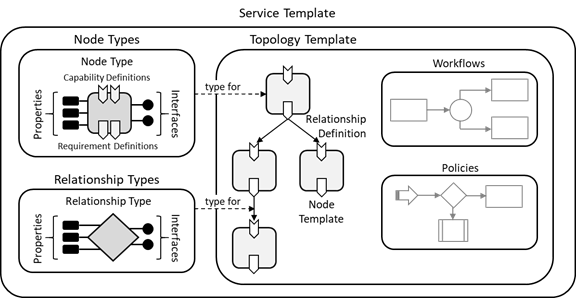
\includegraphics[width=14cm]{tosca_overview}
  \centering
  \caption{Architecture of \gls{toscaacr} and the components of \gls{csaracr} files} %TODO add source: official tosca spec
  \label{image:tosca_overview}
\end{figure}

The last part contained in \gls{csaracr} files are the management plans. They describe the lifecycle of nodes and how to achieve them. Examples are instantiation, configuration and deallocating/uninstallation/deletion (depending on the resource type).
\newline
%TODO add official spec as source
\newline
The standard supports imports with or without namespacing. One potential import is the Simple-Profile extension.
It adds a basic set of such predefined types to the standard, for example the node-types Compute, Webserver, and Webapplication with necessary requirements and capabilities.
\newline
While \gls{toscaacr} does not seem to be very widespread, its origin from OASIS and the many and huge companies backing it and involved in its development make it a very promising standard.
\newline
The architecture of the \gls{csaracr} files and the ability of inclusions and substitutions make it relatively easy to find the corresponding code for a certain component.
\newline
This, and the fact that versioning is not only possible but even required by design make changes in the infrastructure or lifecycles easily managable.


% TODO integrate the following findings into this and the previous sections.

% \url{https://www.slideshare.net/openstackil/heat-tosca}
% HOT == Heat Orchestration Template, YAML only
% came to replace cloud formation syntax
% following the cloudformation limited model
% hot is only for infrastructure creation
%! tosca is application centric by design
%! -> tosca is more universal
%! hot workflow hardcoded in heat engine
%! toscas interfaces allow for any workflow -> no hardcoded workflow
%! tosca to hot translator project developed by ibm, huawei and others -> goal is to describe stack in tosca and use heat
% cloudify uses tosca templates directly
%   soon to use heat to orchestrate infrastructure
%   adds monitoring, log collection, analytics, workflows

%! tosca adopted hot input and output parameters, which took that from cloudformation
% hot added software\_config provider to describe application stack explicitely
% hot adopted tosca relationship syntax and semantics

% \url{https://www.oasis-open.org/committees/download.php/56826/OpenStack%202015%20Tokyo%20Summit%20-%20TOSCA-and-Heat-Translator-TechTalk.pdf}
% "TOSCA-Parser" by IBM, can parse TOSCA Simple Profile in YAML
% "Heat-Translator", maps and translates non-heat (f.e. tosca) templates to hot
%   supports tosca csar
% "Murano" == OpenStack's application catalog that provides application packaging, deployment and lifecycle management - plans to integrate tosca csar

% \url{https://wiki.openstack.org/wiki/Heat/DSL2}
% evolved first heat/dsl and incorporate tosca and CAMP

% Terraform
% - AWS CloudFormation
%   - \url{https://en.wikipedia.org/wiki/RAML\_(software)} -> supported by aws api
% OpenStack Heat -> can use TOSCA
% Cloudify -> uses TOSCA
% ... (see notes)

% Terraform is very similar to tosca, but because its usability is higher and its learning curve is steeper, its a lot more user friendly.

% %TODO application-distribution -> TOSCA CSAR, helm charts, openstack hot packages in murano...
% - CAMP \url{http://docs.oasis-open.org/camp/camp-spec/v1.1/cs01/camp-spec-v1.1-cs01.pdf} , \url{https://en.wikipedia.org/wiki/Cloud\_Application\_Management\_for\_Platforms}
% - Terraform (describes itself as standard: \url{https://www.terraform.io/intro/vs/custom.html} )
% - cloudformation \url{https://www.terraform.io/intro/vs/cloudformation.html}

\subsection{ONLY READ UNTIL HERE}

\subsection{Pulumi}

... %CURRENT

% \item Primary approach \hl{Comparative Study of DSL Tools}
% \item Guarantees provided in case of well-formedness \hl{Comparative Study of DSL Tools} %TODO this also contains "efficiency" like parallelism
% \item Reusability of components \hl{Comparative Study of DSL Tools}
% \item Error proneness and reporting like line number and column offset \hl{Comparative Study of DSL Tools} \hl{Comparing General-Purpose and Domain-Specific Languages - An Empirical Study}
% \item Efficiency: Amount of code for a given case study \hl{Comparative Study of DSL Tools}
% \item Aspects to learn for a given case study or how hard the mental operations are \hl{Comparative Study of DSL Tools} % / learning-curve
% \item Viscosity: How hard it is to make changes/updates \hl{Comparing General-Purpose and Domain-Specific Languages - An Empirical Study}
% \item Hidden dependencies like requiring agents, a dedicated server or a third-party software \hl{Comparing General-Purpose and Domain-Specific Languages - An Empirical Study}
% \item Visibility: How easy is it to find the responsible snippet in the codebase \hl{Comparing General-Purpose and Domain-Specific Languages - An Empirical Study}
% \item Extensibility: Can the language be adapted to environment changes
% \item Maturity (documentation, user-base, community): How good are edge-cases documented and how well is the product established
% \item Ecosystem

\section{Comparison of existing Domain-Specific-Languages}

% --------------------------------------------------------------------------
% ```yaml
% CloudFormation: % https://docs.aws.amazon.com/AWSCloudFormation/latest/UserGuide/updating.stacks.walkthrough.html
%   approach:
%     - declarative
%     - JSON and YAML
%     - typed (AWS::ProductIdentifier::ResourceType, f.e. AWS::EC2::SecurityGroup) - how does the typing system work: field "type" for all components
%     - create "stack update" (execution path), save it in s3-buck or anywhere, then run it. no direct api access?
%     - state is retrieved "live"
%   hidden-dependencies:
%     - AWS only
%   structure:
%     - mappings: % conditional mappings
%       - ... % f.e. different ami images per region and architecture; a lot like a switch statement
%     - metadata: ... % can exist on all levels, contains f.e. information about visual representation
%     - outputs: % viewable on the management console etc.
%       - ... % f.e. Access-URL for an application after installation
%     - parameters:
%       - <variablename>:
%         - Default: ...
%         - Description: ...
%         - Type: ...
%         - minlength, maxlength, regex pattern for strings, ...
%         - Constraintdescription
%     - resources: % only resources are required
%       - WebServer: % valid resource type
%         - type: AWS::EC2::Instance
%         - properties:
%           - UserData: ... % valid values for this resource type
%           - KeyName:
%             Ref: <variablename> % can reference to parameters
%   validation / error reporting:
%     - custom schema validation (?)
%     - only checks if parent language is well-formatted (json,yaml)
%     - additional tools
%       - python cfn-lint as plugin for IDEs or static analysis tool
%       - ruby cfn-nag for static analysis, aimed at security
%       - python taskcat for making a testrun with a template -> integration tests
%     - dry-run possible
%   aspecty-to-learn:
%     - "Fn::..." in JSON, "!..." in YAML -> custom functions like Join, GetAtt
%     - JSON or YAML is required, the graphical designer does only the rawest of work
%       alternatively: use the AWS Cloud Development Kit (AWS CDK) for Typescript, python, java or .net
%     - AWS products, their naming and how each components attributes are named
%   tooling/ecosystem:
%     - integrated in aws-cli
%     - "designer": https://eu-central-1.console.aws.amazon.com/cloudformation/designer/home?region=eu-central-1
%     - any text-editor for JSON/YAML, or use the AWS Cloud Development Kit (AWS CDK) for Typescript, python, java or .net
%     - git pre-commit validation with "cfn\_nag" (https://github.com/stelligent/cfn\_nag) and "taskcat" (https://github.com/aws-quickstart/taskcat)
%   optimizations:
%     - parallel resource creation/updating/deletion, can be controlled with "DependsOn" attribute
%   extensibility:
%     - https://aws.amazon.com/cloudformation/features/: There is a CloudFormation Registry, where third-party sources can provide a template for their app
%   guarantees:
%     - cost calculator: https://calculator.aws/
%     - no guarantee updates work (f.e. insufficient permissions, account quota limit); automatic roll-back on failure
%   reusability of components:
%     - there is the cloudformation registry where apps can be published
%     - "Ref" can reference to other components
%     - nesting of "stacks" is possible
%   Visibility:
%     - predefined structure, splitting into different files possible
%   Viscosity:
%     - updates of the DSL are made by aws
%     - updates to your apps have to be made manually
%     - updates have to be validated manually
%   Consistency:
%     - (probably) pretty high, as developed by one team and being an official product by amazon.
%   notes:
%     - fails if dependend component is neither defined nor already existing
%     - state-monitoring: events; but those are not saying much (only time, type of the event origin (alarm, stack,...), logical ID (custom name), physical ID (instance id), status (f.e. CREATE\_COMPLETE, CREATE\_IN\_PROGRESS), Reason (User initiated))
%     - costs:
%       - AWS::*, Alexa::* and Custom::* are free
%       - 3rd party providers cost stuff
%     - "Naming resources restricts the reusability of templates and results in naming conflict when an update causes a resource to be replaces" [https://aws.amazon.com/cloudformation/faqs/] -> naming is not possible for all components
% ---
% Heat:
%   approach:
%     - declarative
%     - compatible to AWS CloudFormation
%     - OpenStack-native REST API, CloudFormation-compatible Query-API
%     - either cli or api directly
%     - YAML
%     - python app
%     - heat cli accesses heat-api, which sends API-requests via RPC to heat-engine, which does the heavy lifting
%     - python-heatclient lib (== api)
%   hidden-dependencies:
%   structure:
%     - parameters % input parameters, typed
%         image\_type:
%           type: string % every parameter is typed
%           label: Image Type
%           description: Type of instance (flavor) to be used
%           default: m1.small % optional default value
%           %hidden: true % optional attribute to hide secrets from users who request information about the deployed stack
%           constraints:
%             - allowed\_values: [ m1.medium, m1.large, m1.xlarge ]
%               description: Value must be one of m1.medium, m1.large or m1.xlarge.
%             %- allowed\_pattern: "[a-zA-Z0-9.]+"
%           %immutable: true % defines whether the param is updatable
%     - resources % typed, f.e. OS::NOVA::Server
%         my\_instance:
%           type: OS::Nova::Server
%           properties:
%             key\_name: ...
%             image: ...
%             flavor: { get\_param: image\_type }
%           %metadata
%           %depends\_on
%           %update\_policy
%           %deletion\_policy
%           %external\_id
%           %condition
%     - outputs
%         instance\_ip:
%           description: The IP address of the deployed instance
%           value: { get\_addr: [my\_instance, first\_address] } % alternative: get\_file: URL/path and get\_param or get\_resource (like named port)
%           %condition % conditional output is supported
%     %- conditions % declaration of conditions
%     %- parameter\_groups % a declaration of input parameter groups and order
%   validation/error-reporting:
%     - heat template-validate: used to validate a template, with inserting templated values and ignoring specific errors -> feels like dry-run
%   aspects to learn:
%     - YAML
%     - HOT structure, types, functions and how each components attributes are named
%   tooling/ecosystem:
%     - cli
%     - python-lib
%   optimizations: % none?
%   extensibility:
%     - there is NO app catalog (\url{http://lists.openstack.org/pipermail/openstack-operators/2017-July/013965.html}) for heat templates
%   guarantees: % none?
%   reusability of components:
%     - works with cloudformation stuff, and is closely related to it
%   visibility:
%     - see cloudformation
%   viscosity:
%     - see cloudformation (?)
%   consistency:
%     - similar to cloudformation, but with openstack types
%   notes:
%     - imitates AWS Cloudformation on several occasions (types, structures, wording (f.e. stack))
%     - there is a openstack REST-API AND a CFN-API
%     - cli-command names are confusing
%     - "heat" makes the clouds rise
% ---
% Terraform:
%   approach:
%     - declarative
%     - plugins; allow for different providers
%     - dependencies possible
%     - state of real infrastructure in "state file" == source of truth; remote state backend feature; file is refreshed on every "terraform apply"
%     - terraform cloud to prevent race conditions
%     - init command downloads and installs required provider plugins
%     - creates execution plan
%     - own format (HCL), but JSON is also supported
%     - architecture
%       - core does state mgmt, constructs resource graph and discovers and communicates with plugins via rpc
%       - plugins are binaries as well and are invoked via rpc
%       - plugins should initialize included libraries to make api calls, authenticate and define resources that map to services and run commands/scripts
%       - terraform init checks configuration files to determine which plugins are necessary (and saves current version of plugin until init is ran again)
%       - providers are downloaded from tf-registry, but network- or file-system-mirror can be configured
%       - if no provider is set, local lookups are done by default as well (both global and current dir)
%       - dev overrides possible, without failsafes
%   hidden-dependencies:
%     - HCL requirement just adds another layer, and migration between clouds is still a lot of manual work
%     - cloud-specific cli (like aws-cli)
%     - terraform init downloads additional modules (but internet connection is already required for most providers)
%     - sometimes requires the cloud-specific cli as well
%   structure:
%     - main.tf ; contains:
%       - terraform configuration/settings (provider, f.e. aws-cli)
%       - provider-specific configuration like region, profile
%       - resources -> 'resource "<type>" "<name>" {...}' -> id == <type>.<name>
%     - variables.tf ; contains
%       - input variables (typed, via param), used with 'var.<variablename>'
%     - outputs.tf ; contains which values should be output when apply is ran
%   validation/error-reporting:
%     - `terraform fmt`: format configuration
%     - `terraform validate`: validate configuration
%   aspects to learn:
%     - HCL (complete "language", similar but still different to JSON) -> alternatively, JSON can be used as well
%     - provider-specific resources and their attributes
%   tooling/ecosystem:
%     - terraform cli
%     - terraform registry for 3rd party
%   optimizations:
%     - parallel execution of actions whenever possible (can even be limited)
%   extensibility:
%     - plug-ins / external modules
%   guarantees:
%     - none - no rollback when in state-migration and facing an error (https://news.ycombinator.com/item?id=19472485)
%   reusability of components:
%     - providers, plug-ins \& modules
%   visibility:
%     - all *.tf files are considered and read, so it is possible to split as much as you want - in the same directory
%     - components in subfolders should be made tf-modules
%       - at least one module; called root-module in the main dir
%       - modules can be called multiple times
%       - modules can have input variables, which can be passed from the caller (used with 'module.<modulealias>.<variabelname>')
%       - modules are defined by source-uri, which might be a relative dir-path, http, git, registry, s3-bucket ...
%     - visibility depends on module-structure
%   viscosity:
%     - updates in all directions seem to be quite easy or at least the tooling is there - for debugging as well
%   consistency:
%     - providers and modules are developed by different people, so they tend to be inconsistent.
%     - overall structure is predefined
%   notes:
%     - track resources with state
%     - resusable components == modules
%     - tells when resources are updated and when they are replaced and on the latter which attribute causes the replacement
%     - Problem with statefile; changed region after deployment, then went for destroy -> terraform didnt find the deployment and deleted it from the statefile after resetting the value, making it undeletable. Manually restoring the statefile was necessary to be able to destroy the deployment.
%     - purpose of the statefile:
%       - mapping between non-named resources to generated name
%       - how should terraform know to delete a resource (and dependencies and their destruction order) when its not in the config file any more?
%       - for larger infrastructure, querying everything for each action is too much overhead and might become a problem with rate limits
%       - statefile is only useful for single-user usage, for teams a remote-state-backend is used like tf-cloud, consul, aws-s3, azure blob, gcp storage, alibaba cloud etc
%         - latest state present, resource locking == state locking, so no corruption during writing
%       - local state contains plain initial passwords, remote state might be encrypted
%       - only tf-internal use recommended, use json flag for output commands
%     - multiple environments/workspaces sometimes supported; dev, prod, local etc.
%     - wants every external file to be translated to own file-format, f.e. dockerfile \url{https://learn.hashicorp.com/tutorials/terraform/docker-build?in=terraform/docker-get-started}
% ---
% Tosca/cloudify:
%   approach:
%     - webapp, manager with REST-API, accessed via webgui and/or cli
%     - manager, database and messaging queue -> either hosted on one box (vm/container) or clustered (all services on all nodes or each service on different node)
%       - manager:
%         - event-stream processing
%         - secured requests
%         - metric/logs/events queueing
%         - aggregation and analysis
%         - task execution/queueing, can be automated based on live streams of events or aggregated data
%         - interaction with cloudify agents
%     - has optional agents installable via ssh/winrm or f.e cloud-init or plugin (temporary download link for the install script) or agent preinstalled in image or no agent at all
%       - execute orchestration operations locally
%       - collect metrics and report them to manager
%     - blueprints == app-description
%       deployment == instance of app (but with its own scaling etc)
%   hidden-dependencies:
%     - dedicated manager-server, global for complete infrastructure is needed (partial access is done via permissions...)
%   structure:
%     - how to actually write components and templates is hard to find in the docs -> \url{https://docs.cloudify.co/latest/developer/writing_plugins/creating-your-own-plugin/#writing-plugin-operations}
%   validation/error-reporting:
%     - ide linting \& type validation
%   aspects to learn:
%     - YAML
%     - TOSCA/cloudify standard
%   tooling/ecosystem:
%     - ide-autocompletion
%     - examples for aws, terraform, azure, gcp and openstack, but all with predefined code (since its hard to create that)
%   optimizations:
%     - parallelism, resource graph
%   extensibility:
%     - plugins can be extended, and written by yourself, blueprints
%   guarantees: none?
%   reusability of components:
%     - plugins
%     - blueprints
%   visibility:
%     - depends on structure of project
%   viscosity:
%     - updates don't seem to considered properly somehow
%   consistency:
%     - completely different for different providers, even the api-call is completely different
%   notes:
%     - see notes.md
% ---
% Tosca/simple-profile:
%   approach:
%     - YAML
%     - namespaced imports (of type definitions) possible
%       prefixes:
%       - tosca: from tosca-definitions
%       - <none>: try to find in tosca namespace first, then lookup in current file (tosca.nodes.Compute == Compute)
%       - <namespaced-import>: imported file, alias for namespace defined there
%     - types, automated type-matching (same name for instances of different types -> tosca automatically matches correct type)
%     - property types:
%       - string (default)
%       - integer
%       - float
%       - boolean
%       - timestamp
%       - null
%     - other types:
%       - range [lower, upper|UNBOUNDED] -> can be used for template values, like port-numbers etc ("constraints")
%       - list [ elem1, elem2, ...] == yaml-list (isnt this normal yaml stuff?) f.e.
%         something:
%           type: list
%           entry_schema:
%             description: ...
%             type: <sometype>
%             [constraints]: ..<list>..
%       - map: normal key-value pair, shorthanded with {}
%       - scalar-unit: <scalar> <unit> % whitespace between is allowed but not required, case-insensitive
%         types:
%         - scalar-unit.size == 1 B, ..., 2 TiB
%         - scalar-unit.time == 1d, 2h, ..., 3ns
%         - scalar-unit.frequency == 1Hz, ..., 5GHz
%         - scalar-unit.bitrate == 1bps, ..., 2GBps, 3TiBps
%       - node-states:
%         - initial: not created, only defined in template
%         - creating -> created
%         - configuring -> configured
%         - starting -> started
%         - stopping -> configured
%         - deleting -> not longer tracked
%         - error
%       - relationship-states: % -> would require additional states?
%         - initial: relationship is not yet created, only exists in template
%       - special directives:
%         - substitute: mark node template as abstract, orchestrator must substitue with appropriate template
%         - select: mark node template as abstract, orchestrator must select a node of this type from its inventory (based on defined constraints ("node_filter"))
%       - network-names: % used in tosca.capabilities.Endpoint capability type
%         - PRIVATE
%         - PUBLIC
%     - reusable modeling definitions:
%       - description: <string>
%       - metadata: <map>
%       - constraint: [<operators>] % usable on integer, float, timestamp, string, version and scalar-unit % "schema" is special
%       - <property-filter-definition>, f.e. % see structure
%         node_filter:
%           properties:
%             - <something>
%           capabilities: % first checked whether cap is a symbolic name and second if it is a type name
%             - <something>
%       - repository: defined by [ description, url, credential ], but only url is required
%       - <artifact_name>: defined by [ type, file, [deploy_path,checksum,...]] % could contain simple txt-files or disk image with checksum (example in spec at 3.6.7.3)
%       - imports: [uris] % see prefixes and namespaces
%       - <property_name>: [ type, description, required, default, status (supported), constraints, key_schema, entry_schema, external-schema, metadata ]
%       - <attribute_name> [ type, description, default, status, key_schema, entry_schema ]
%       - output_name: [ [SELF|SOURCE|TARGET], attribute_name, ...] % named output
%       - operation implementation, <operation_name>: [ primary (f.e. if primary script in scar file), dependencies (other operations), operation_host ([SELF|HOST|SOURCE|TARGET|ORCHESTRATOR]), timeout] 
%       - operation, <operation_name>: [ description, implementation (<operation implementation>), inputs, outputs ] % execute script or command
%       - (similar to operations) notification, <notification_name>: [ description, implementation, outputs ]
%       - interface: [ inputs, operations, notifications ]
%       % form here onwards, only the typenames are listed
%       - event filter
%       - trigger definition
%       - activity
%       - set state of node by activity
%       - call operation activity
%       - inline workflow
%       - assertion
%       - condition clause (and, or, not, assert)
%       - workflow precondition
%       - workflow step
%       % type-specific definitions:
%       - entity type schema
%       - capability
%       - requirement
%       - artifact
%       - interface type
%       - data type % f.e. phone number
%       - capability type
%       - requirement type
%       - relationship type
%       - group type
%       - policy type
%       % template-specific definitions
%       - capability assignment
%       - requirement assignment
%       % node template
%       % relationship template
%       % group definition
%   hidden-dependencies:
%   structure: % how tosca works https://docs.oasis-open.org/tosca/TOSCA/v2.0/csd03/TOSCA-v2.0-csd03.html#_Toc56506180
%     - my_node_template
%         requirements:
%         - host:
%             node_filter:
%               capabilities:
%               - host:
%                   properties:
%                   - num_cpus: { in_range: [1,4] }
%                   - mem_size: {greater_or_equal: 512MB }
%   validation/error-reporting:
%   aspects to learn:
%     - YAML (since v2)
%     - tosca % there is tosca v1 and v2, but v2 seems to be a copy of v1 so far... but it feels a bit more concise/readable in its structure | v1 == xml, 2v == yaml
%     - tosca simple profile % actually, this is the more important standard, tosca itself is about more abstract stuff
%     - one-time setup of "everything-as-a-service", then only the derived types etc are required to learn
%   tooling/ecosystem:
%     - winery, vinothek -> docker image not working
%     - (cloudify)
%   optimizations:
%     - none?
%   extensibility:
%     - very flexible, as the standard can be extended a lot
%   guarantees:
%     - none?
%   reusability of components:
%     - type definitions can be reused
%     - template definitions can be reused
%     - csar application archive format
%   visibility:
%     - definitions, types, plans, etc feel hard to distinguish
%   viscosity:
%     - definitions have version-fields
%     - updatability seems great so far.
%   consistency:
%     - really great
%   notes:
%     - where does yaml-schema fit in? this seems to define its own meta-schema?
%     - cloudify and alien4cloud used tosca before spec reached final state: https://gitter.im/ystia/yorc?at=5e3b29bfbfe65274eae0f3d0
% ---
% % really strange documentations:
% ystia / yorc : only for compute, disk, vpc and public ip (but on many providers like aws, gcp, openstack, ...) \& k8s
% alien4cloud : many providers like openstack, slurm, hosts pool, gcp, aws, k8s
% ---
% there are two types so far:
% - cli, where the dsl is "not perfect" (cloudformation, heat)
%   - hcl vs yaml https://xkcd.com/927/
%     - (?) hcl to json is hard, yaml to json is easy
%     - hcl is optimized for terraform and other hashicorp products
%     - hcl tooling isn't good (even basic linting doesnt exist/work)
% - "perfect dsl" without cli tools and undefined everything as a service (tosca)
% potential main goals:
% - implement cli tool for tosca(-extension) (and design corresponding everything-as-a-service reference definitions)
%   - init command generates definitions
%   - minify removes unused definitions
% - implement tosca parser for terraform/hcl
% additional goals possible:
% - implement one or two reference providers (direct)
% - 
% ---
% implementation details (terraform):
% - grpc as rpc between modules / for plugin-architecture, requires server and clients to be running in parallel - how to start on demand?
%   - ssl/tls by default
%   - grpc-web might enable gui-stuff
% - statefile? namespacing for performance?
% ```
% ---------------------------------------------------------------------------------------------------------------------------------------------------------

% %TODO how does deprovisioning work
% %TODO how are existing resources referenced
% %TODO how to handle secrets in outputs
% %TODO how to handle secrets in templates
% %TODO noecho in cloudformation still shows stuff in output, metadata etc -> how to provide a secure way not giving away credentials?

%TODO -> how can those standards be improved? And what can be added?

\section{Everything-as-a-Service}
- can openstack do all of this?
  - stability
  - legacy code
  - complexity
- Rackspace-as-a-Service; will-on-prem die? ("Why on-prem won't die") no, security of data, costs, privacy, pressure/trust, (with or without pdu, usc, ups)
- Metal-as-a-Service; vs VM-as-a-Service (vps), noisy neighbour, vSphere AutoDeploy, Ironic, tinkerbell, ipv6, which os, ipmi, kernel/firmware integrity, zones, pdu, psu, rack, sdn
- Network-as-a-Service; topology, vlan, sdn, both on hw and sw layer
- DNS-as-a-Service; global or not? via k8s?
- Hypervisor-as-a-Service; esxi, kvm (used by aws, gcp (no qemu)), node-size, vm-size, compare to metal-as-a-serice (differentiate)
- Compute-as-a-Service; vm-as-a-service, vps
- Encryption-as-a-Service: ram, disk, network on host/node-level (TPM?)
- Storage-as-a-Service; alternative to rook, hyper-converged vs dedicated (SVC by IBM), sds, both on hw and sw layer
- IAM-as-a-Service; webauthn with yubikey, cloud-iam, 3rd-party iam like github oauth (openstack iam? ad necessary? why no ad join for nodes? -> linux, ephemereal, cattle)
- k8s-as-a-Service; which os, in-memory-os, cluster-api (gardener, how to configure nodes? Terraform, ansible, cloud-init, ignite), why multi-tenacy via multi-cluster?
- IaC-as-a-Service; generation/compliance with OPA, CRD-like formal description, check GCP, AWS, Azure and Openstack for common ground
- secrets-as-a-Service; turtles all the way down presentation, SCM, orchestration, Secrets-as-a-service (hashicorp vault?)
meta/mgmt
- bare-metal-marketplace

\section{Example reference infrastructure} %TODO multiple?
- Are VMs dead? / will containers replace them completely? (/ the case for bare-metal)
  - isolation level
  - comparison of bare-metal approach vs vSphere and/or OpenStack approach
  - constraints like
    - Workload comparison; are there workloads which cannot run in containers and require VMs?
    - minimum machine size defines minimum cluster size and therefore introduces unused resources (when going for temporary k8s-clusters for devs)
  - -> VMs make sense! What about their overhead? They need "zone/node affinity" as well
  - kubevirt?
- common components:
  - public or not (dns / routing)
  - load-balancer / ha
  - persistent or not / storage
  - web-service / api -> should mirror most applications and uses other components
    - db-api
    - web-api
    - REST(ful)-API / CRUD (create, read, update, delete or in HTML: put, get, put, delete, or combine with post)
    - ACID
  - identity / email ?
  - function-as-a-service / serverless -> special case
  - trend:
    - \url{https://en.wikipedia.org/wiki/Resource-oriented_architecture}, \url{https://en.wikipedia.org/wiki/Resource-oriented_computing}, \url{https://en.wikipedia.org/wiki/Service-oriented_architecture}, \url{https://en.wikipedia.org/wiki/Web-oriented_architecture}
    - include example in reference architecture?
    - open data protocol \url{https://en.wikipedia.org/wiki/Open_Data_Protocol}
    - \url{https://en.wikipedia.org/wiki/RSDL}
    - \url{https://en.wikipedia.org/wiki/OpenAPI_Specification} (formerly swagger)
- %TODO where does kubernetes fit in?
- hw-security
  - limit available OS images; optimize those for own hw -> less generic drivers, no overall driver-issues, less to support
  - three installation flavors:
    - install with pxe
    - install with attached iso (via ipmi or hypervisor)
    - preinstalled virtualdisk (only for vms) -> azure
    - ibm supports only attached iso: \url{https://cloud.ibm.com/docs/bare-metal?topic=bare-metal-bm-mount-iso}
  - firmware
    - some hw supports firmware flashing from os level which can result is hardware damage (increasing voltage etc)
    - either on provision or deprovision task update all firmwares to latest official firmware versions (no matter what was installed before - even if it seems to be that already)
      - on deprovisioning makes more sense, it saves time when provisioning new nodes.
    - upgrades can then happen globally (for all "unused" nodes) and used nodes can be migrated by users (or not...)
    - allow to select which firmware version to have flashed
      - latest is default
      - fix them to current latest version after latest was used
  - \url{https://docs.microsoft.com/en-us/azure/baremetal-infrastructure/concepts-baremetal-infrastructure-overview}
    - ? bare metal is ISO 27001, ISO 27017, SOC1 SOC2 compliant
    - RHEL and SLES only
    - ECC vs EDAC (Error Detection And Correction) module; ECC is in hardware, EDAC in software, when both enabled, they can conflicts, with unplanned shutdowns of a server.
    - managed bare metal; up to OS is managed, then the customer is responsible

\section{Issues with existing standards and frameworks}
- no comparison of iac dsls
- not enough effort to integrate with other tools / dsls / clouds (vendor-lock-in seems desired)
- either no proper standard (vendor-specific) or not enough support for multiple vendors -> everyone reinvents the wheel and wants to establish the own work as industry-standard
- %TODO: propose solution / new approach -> integrate all, search common ground, can tosca solve this?

%TODO market at bottom of iac
